\documentclass[11pt]{article}
\usepackage[margin=1in]{geometry}
\usepackage{mathpazo}
\usepackage{amsmath,amssymb,amsthm}
\usepackage[expansion=false]{microtype}
\usepackage{xcolor}
\usepackage{booktabs,tabularx,array,longtable}
\usepackage{enumitem}
\usepackage{listings}
\usepackage{graphicx}
\usepackage{tikz}
\usetikzlibrary{positioning,arrows.meta,fit,calc,backgrounds,shapes.geometric}
\usepackage{xurl}
\usepackage[hidelinks]{hyperref}
\usepackage[htt]{hyphenat}

\theoremstyle{definition}
\newtheorem{requirement}{Requirement}
\newtheorem{principle}{Principle}
\newtheorem{decision}{Open decision}
\newtheorem{obligation}{Obligation}
\newtheorem{finding}{Finding}
\newtheorem{resolution}{Resolution}
\theoremstyle{remark}
\newtheorem{remark}{Remark}

\newcommand{\MUST}{\textsc{must}}
\newcommand{\MUSTNOT}{\textsc{must not}}
\newcommand{\SHOULD}{\textsc{should}}
\newcommand{\SHOULDNOT}{\textsc{should not}}
\newcommand{\MAY}{\textsc{may}}
\newcommand{\code}[1]{\texttt{#1}}
\newcommand{\Nd}{F1R3Node-Rust}
\newcommand{\Em}{Embers}
\newcommand{\Sky}{F1R3Sky}
\newcommand{\Gz}{F1R3Gaze}
\newcommand{\Pt}{the Portal}
\newcommand{\PT}{The Portal}
\setlength{\emergencystretch}{3em}
\renewcommand{\arraystretch}{1.15}

\definecolor{cm}{RGB}{90,110,90}
\definecolor{sky}{HTML}{3FA9F5}
\definecolor{ylw}{HTML}{F3D630}
\lstset{
  basicstyle=\ttfamily\small,
  commentstyle=\color{cm}\itshape,
  columns=fullflexible,
  keepspaces=true,
  frame=single,
  framerule=0.3pt,
  rulecolor=\color{black!30},
  xleftmargin=4pt,xrightmargin=4pt,
  aboveskip=6pt,belowskip=6pt,
  breaklines=true,
  upquote=true
}
\lstdefinelanguage{Rho}{
  morekeywords={new,in,for,contract,match,if,else,bundle,bundle0,Nil,true,false,not,and,or},
  sensitive=true,
  comment=[l]{//},
  morestring=[b]",
  morestring=[b]`
}
\lstdefinelanguage{Json}{morestring=[b]"}

\title{%
  
\includegraphics[width=0.36\textwidth]{ffio-logo.pdf}\\[18pt]
  \textbf{The F1R3Games Portal: Design Document}\\[4pt]
  \large Single sign-on with a built-in wallet, galleries of game plays,\\
  launching games, and invitations, on a \Nd{} shard\\[6pt]
  \normalsize Version 0.1 (draft for review)}
\author{Lucius Gregory Meredith\\
\small CEO, F1R3FLY.io, and Chief Science Officer, F1R3FLY Industries}
\date{5 October 2026}

\begin{document}
\maketitle

\begin{abstract}
\noindent
This document designs the F1R3Games Portal: the single web entry point to the
F1R3Games suite (F1R3Pix, F1R3Beat, F1R3Ink, F1R3SideChat, F1R3Skein, and the games
that follow them). A person arrives with nothing but a browser, creates or imports a
secp256k1 private key, and from then on is signed on to every game. A built-in wallet
holds the key, pays for every deploy the person makes, shows balances and history,
and moves funds. The person can browse the gallery of past plays of every game
(including, for F1R3Skein, the separate galleries of tunes and of performances),
launch a new instance of any game, and bring other people into it by sharing her
contacts with the Portal and sending invitations.

The backend is a \Nd{} shard, reached through the \Em{} service pattern. The design
is written to \emph{conform}: to \Nd{} first (its HTTP and gRPC interface, its system
contracts and their current names, its node roles and its proposing policy), then to
\Em{} (its service layering, its prepare/sign/send protocol, its typed rendering of
Rholang, its wallet API and client SDK), then to \Sky{} (its wallet file format and
its wallet flows). The earlier F1R3Games work, the portal prototype, the per-game
\code{Shard/} services and the contact dialogues, is treated as research: its
concepts are carried forward, its code is not. The design is grounded in a review of
\Nd{} \code{master} at \code{95be0d4} and \code{feature/cost-accounted-rho} at
\code{068d51c}, \Em{} at \code{28e50d4}, \Sky{} at \code{57dcae5}, F1R3Games
\code{main} at \code{ed61943} and \code{v2} at \code{18a675a}, \Gz{} at
\code{f6ee26a}, and ign1t10n at \code{46faa56}.
\end{abstract}

\tableofcontents
\newpage

%======================================================================
\section{Scope and conventions}\label{sec:scope}

\subsection{What the Portal delivers}

After this design is implemented, a person with an ordinary web browser can:

\begin{enumerate}[leftmargin=*,itemsep=2pt]
\item \textbf{Sign on with a private key.} Create a new secp256k1 key, or import one
  saved by \Sky{} or \Gz{}, and use it as the sole credential for every game. There
  are no passwords held by any server and no email-based accounts.
\item \textbf{Use a built-in wallet.} See the balance and history of the address the
  key controls, receive funds, send funds, see what each game has cost, and approve
  or refuse every charge before it is made.
\item \textbf{Browse previous games.} Scroll the gallery of plays of any game, or a
  feed across all games, without launching anything and without signing on.
\item \textbf{Launch a game.} Start a new instance of any game, which appears on the
  shard as an object the person hosts, and open the game on it.
\item \textbf{Invite others.} Share contacts with the Portal (from a file, a
  platform's contact picker, or by hand), choose whom to invite, and deliver
  invitations through the person's own channels. An invitation, when redeemed, brings
  the invitee into the instance, creating a key for them if they have none.
\end{enumerate}

\subsection{Non-goals for this version}

\begin{itemize}[leftmargin=*,itemsep=2pt]
\item The internal mechanics of any game. Each game owns its rules, its on-chain
  state and its user interface; the Portal owns identity, payment, instances,
  galleries, invitations and the contract between itself and the games
  (\S\ref{sec:games}).
\item Custodial accounts or key recovery by the operator. The key is the person's,
  as it is in \Sky{} and \Gz{}.
\item Fitness and selection for the evolutionary games. The Portal records
  engagement (\S\ref{sec:engagement}); how F1R3Skein and F1R3Beat turn engagement
  into reproduction is theirs to decide.
\item Delivery of invitations by an operator-run mail server or bot. The design
  leaves room for it (\S\ref{sec:delivery}) and does not depend on it.
\item The f1r3lang rendition of the Portal for \Gz{}. It is sketched as a later phase
  (\S\ref{sec:gaze}).
\end{itemize}

\subsection{Order of authority}\label{sec:authority}

Where sources disagree, this design resolves the disagreement in a fixed order:

\begin{enumerate}[leftmargin=*,itemsep=2pt]
\item \textbf{\Nd{}} \code{master}: the node's API reference (\code{docs/node}), its
  system processes (\code{rho\_runtime.rs} in the interpreter), its system
  contracts (\code{casper/src/main/resources}) and its node roles. Features present
  only on \code{feature/cost-accounted-rho} are designed \emph{for}, never depended
  \emph{on}, until they reach \code{master}.
\item \textbf{\Em{}}: the service layering in \code{packages/embers}, the
  prepare/sign/send protocol in \code{api/common.rs}, the typed Rholang rendering in
  \code{packages/firefly-client}, the environment-contract pattern in
  \code{templates/common/insert\_signed.rho}, the wallet API, and the client SDK
  \code{@f1r3fly-io/embers-client-sdk}.
\item \textbf{\Sky{}}: the wallet key file, the create-and-download and
  upload-to-add wallet flows, and the use of the \Em{} SDK from a React client.
\item \textbf{\Gz{} and ign1t10n}, where they have settled a question the three above
  leave open (the signing-safety rules of \Gz{}'s wallet; ign1t10n's local shard
  topology).
\item \textbf{The earlier F1R3Games work}, as research only.
\end{enumerate}

\subsection{Conventions}

\MUST, \MUSTNOT, \SHOULD{} and \MAY{} are used in the sense of RFC~2119. ``Address''
means a F1R3Cap address as the \Em{} SDK derives it from a secp256k1 public key.
``Deploy'' means a signed \code{DeployData} as \Nd{} accepts it at \code{POST
/api/deploy}. ``Validator'' and ``observer'' mean a bonded node and a read-only node
respectively. ``Instance'' means one play of one game: what a player launches and
invites others into. ``Play record'' means the gallery entry an instance, or a part
of one, leaves behind.

%======================================================================
\section{Requirements}\label{sec:req}

\begin{requirement}[Single entry point]\label{req:entry}
All games \MUST{} be reachable from one Portal, and a person signed on to the Portal
\MUST{} be signed on to every game launched from it without a further sign-on step.
\end{requirement}

\begin{requirement}[Key-based sign-on]\label{req:key}
The only credential \MUST{} be a secp256k1 private key. The Portal \MUST{} create
keys and import keys in the \Sky{} wallet file format, and \MUST{} export keys in
that format, so that one key works in the Portal, \Sky{} and \Gz{}.
\end{requirement}

\begin{requirement}[Built-in wallet]\label{req:wallet}
The Portal \MUST{} contain a wallet that shows balance and history, receives and
sends funds, and signs and pays for every deploy the Portal or a game makes on the
person's behalf, after the person's consent or within an allowance the person has
set.
\end{requirement}

\begin{requirement}[Galleries]\label{req:gallery}
Every game \MUST{} have a gallery of plays, browsable from the Portal without
launching the game and without signing on. F1R3Skein \MUST{} have two galleries,
tunes and performances, cross-linked.
\end{requirement}

\begin{requirement}[Launch]\label{req:launch}
A signed-on person \MUST{} be able to start a new instance of any game, and the
instance \MUST{} exist on the shard before any invitation to it is issued.
\end{requirement}

\begin{requirement}[Contacts and invitations]\label{req:invite}
A person \MUST{} be able to share contacts with the Portal and invite them to an
instance or to the platform. One contact dialogue \MUST{} serve every game, except
that the F1R3Skein browser does not use it.
\end{requirement}

\begin{requirement}[The shard is the backend]\label{req:shard}
Every durable fact about players, instances, plays, invitations and engagement
\MUST{} live on the \Nd{} shard. Any service in front of the shard \MUST{} be
stateless in the sense that it can be destroyed and rebuilt from the shard and its
own configuration.
\end{requirement}

\begin{requirement}[Open to new games]\label{req:open}
Adding a game \MUST{} require registering it, not changing the Portal.
\end{requirement}

\begin{requirement}[Conformance]\label{req:conform}
The Portal \MUST{} use \Nd{}'s interfaces and system names as they are on
\code{master}, \Em{}'s protocol and libraries, and \Sky{}'s wallet format, and
\MUSTNOT{} introduce a parallel mechanism where one of these already provides one.
\end{requirement}

%======================================================================
\section{Findings}\label{sec:findings}

These are the facts the design rests on. The first group fixes what the Portal must
conform to; the second records what the earlier F1R3Games work taught and what it got
wrong, so that the mistakes are not repeated.

\subsection{What the Portal conforms to}

\begin{finding}[Deploys]\label{f:deploy}
\Nd{} accepts deploys at \code{POST /api/deploy} on validators only. The body is
\code{data} (\code{term}, \code{timestamp}, \code{phloPrice}, \code{phloLimit},
\code{validAfterBlockNumber}, \code{shardId}, and an optional
\code{expirationTimestamp}), \code{deployer} (hex public key), \code{signature} and
\code{sigAlgorithm} \code{"secp256k1"}. The response is the deploy id. Deploy
status is at \code{GET /api/deploy/\{id\}} and
\code{GET /api/deploy-finalization-status/\{sig\}}
(\code{docs/node/api-reference.md}).
\end{finding}

\begin{finding}[Reads need an observer]\label{f:observer}
\code{explore-deploy}, \code{estimate-cost}, \code{balance}, \code{registry} and the
validator queries run only on read-only nodes; a validator answers
\code{400 readonly\_node\_required}. \code{GET /api/status} reports
\code{isValidator} and \code{isReadOnly}. An exploratory deploy returns what is sent
on the \emph{first} unforgeable name of its \code{new}, which must carry no URI.
\end{finding}

\begin{finding}[Names can be known before a deploy]\label{f:prepare}
\code{POST /api/prepare-deploy} with a deployer, a timestamp and a count returns the
unforgeable names that deploy will create, and the validator's next sequence number
for \code{validAfterBlockNumber}. A client can therefore know an object's identity on
the shard before the deploy that creates it is accepted.
\end{finding}

\begin{finding}[Events]\label{f:events}
\code{/ws/events} streams \code{block-created}, \code{block-added},
\code{block-finalised} (each with the deploys it contains: id, cost, deployer,
errored) and, on observers only, \code{transfers-available}.
\end{finding}

\begin{finding}[Proposing]\label{f:propose}
Propose is an admin operation (\code{POST /api/propose} on port 40405; gRPC
ProposeService on 40402). Validators propose on their own when heartbeat proposing is
enabled (\code{--heartbeat-enabled}). \Em{} calls propose once, at bootstrap, after
deploying its environments (\code{packages/embers/src/main.rs}).
\end{finding}

\begin{finding}[System names on \code{master}]\label{f:urns}
\raggedright
The runtime registers \code{rho:vault:address}, \code{rho:system:deployerId:ops},
\code{rho:deploy:data}, \code{rho:block:data}, \code{rho:registry:ops},
\code{rho:crypto:blake2b256Hash}, \code{rho:crypto:secp256k1Verify},
\code{rho:io:devNull} and \code{rho:execution:abort}; system contracts include
\code{rho:vault:system} (\code{SystemVault}: \code{findOrCreate},
\code{deployerAuthKey}, \code{unforgeableAuthKey}, \code{transfer}),
\code{rho:vault:multiSig}, \code{rho:lang:treeHashMap},
\code{rho:registry:insertSigned:secp256k1} and \code{rho:registry:lookup}. The
\code{rho:rev:*} and \code{rho:rchain:*} names used by older code are gone.
\end{finding}

\begin{finding}[Capabilities and offered funding are not on \code{master}]\label{f:branch}
The capability registry \code{rho:system:capabilities} (bounded-use handles) and the
offered-funded deploys with private purses (\code{vault\_payer.rs},
\code{SystemVault.transferBatch}, settlement receipts) exist on
\code{feature/cost-accounted-rho}; the latter's own proposal records that final
qualification is pending. Neither is on \code{master}.
\end{finding}

\begin{finding}[\Em{} is the service pattern]\label{f:embers}
\Em{} is a stateless Rust service (poem-openapi) laid out as
\code{api/<domain>}, \code{domain/<domain>}, \code{blockchain/<domain>},
\code{templates/<domain>/*.rho}. Each domain deploys a versioned environment through
\code{rho:registry:insertSigned:secp256k1} under its own environment key,
re-initialising only when the on-chain version is lower; state lives in
\code{treeHashMap}s; the caller's address is derived inside the contract from
\code{rho:deploy:data} and the vault-address \code{fromDeployerId} operation. Writes
use a two-step protocol: \code{/prepare} returns the deploy bytes the server rendered
plus a token (a JWT binding a hash of the request and response, valid one day);
the client signs the bytes and posts them with the token to \code{/send}. The key
never reaches the server. Templates are rendered by \code{firefly-client}, whose
typed \code{Value} (tuple, list, set, map, nil, bool, int, string, bytes, URI)
renders literals; user strings never reach a template as raw text.
\end{finding}

\begin{finding}[\Em{} already has the wallet and versioned records]\label{f:emberswallet}
The wallets domain serves \code{GET /:address/state}, \code{POST
/transfer/prepare|send}, \code{POST /boost/prepare|send} and \code{GET
/:address/deploys}. The agents and OSLF domains store per-address records with
versions and a \code{"latest"} alias, and project headers in list views by omitting
the heavy field. The testnet domain funds test wallets (\code{POST /testnet/wallet}).
\end{finding}

\begin{finding}[\Sky{}'s wallet]\label{f:sky}
\Sky{} creates a wallet with the SDK's \code{PrivateKey.new()} and immediately saves
it as \code{<address>.json} (\code{serializeKey}); it adds a wallet by uploading that
file (\code{deserializeKey}); it keeps wallets only in memory, so a reload requires
the file again; each wallet carries an \code{EmbersApiSdk} bound to its key. The file
is \code{\{"keyType":"secp256k1","value":"<64 hex>","valueFormat":"hex"\}}, as \Gz{}
also documents and tests.
\end{finding}

\begin{finding}[\Gz{}'s signing-safety rules]\label{f:gaze}
\Gz{}'s wallet decodes prepared bytes strictly, checks shard id and that
\code{phloPrice}~$\times$~\code{phloLimit} is within a fee cap, requires a transfer
term to be exactly \Em{}'s template with the user's own values, and refuses any
program that binds the deployer's identity, from which a program could obtain the
vault's authority and spend.
\end{finding}

\begin{finding}[Name drift in \Em{}]\label{f:drift}
\raggedright
\Em{}'s templates (last commit February 2026) bind \code{rho:rev:address}, and
\Gz{}'s allow-list names \code{rho:rev:address} and \code{rho:rchain:deployId};
\code{master} has \code{rho:vault:address} and \code{rho:system:deployId}. By the
order of authority, the Portal's templates use the \code{master} names, and the
\Em{} templates the Portal relies on must be brought to them
(Obligation~\ref{ob:drift}).
\end{finding}

\subsection{What the earlier F1R3Games work teaches}

\begin{finding}[Concepts worth keeping]\label{f:keep}
The prototype established the shape of the experience: a landing page, identity
creation and import, a dashboard of game cards each offering \emph{launch} and
\emph{gallery}; a sigil avatar derived from the address; a contact-import step with
sources (email, CSV, platform handles, manual) feeding an invite carousel and a lobby;
F1R3Skein's distinction between tunes and performances; SideChat's free reader tier.
All of these are kept.
\end{finding}

\begin{finding}[Mistakes not to repeat]\label{f:mistakes}
\begin{enumerate}[leftmargin=*,itemsep=1pt]
\item Identity used ECDSA P-256 keys and the artifact storage shim, not secp256k1
  and a shard.
\item Accounts, contacts, sessions and invites lived on public string-named channels
  (\code{@"f1r3-accounts"} and so on), consumed and re-sent whole: any deployer could
  overwrite them, and every writer contended for one datum.
\item Contacts, which are other people's personal data, were written to the chain in
  plaintext.
\item Rholang was built by string interpolation of user input.
\item No game had a notion of an instance; each kept one global state.
\item Clients called propose.
\item Shared code was shared by copying (\code{key-management.ts}, with a Python
  slice in TypeScript, duplicated across games).
\end{enumerate}
\end{finding}

\subsection{How conformance closes the open questions}

The review of 5 October 2026 left several questions open. Taking \Nd{}, \Em{} and
\Sky{} as the authorities closes them:

\begin{resolution}[Key type and format]
secp256k1, F1R3Cap addresses, \Sky{}'s key file, all through the \Em{} SDK
(Findings~\ref{f:deploy}, \ref{f:sky}).
\end{resolution}

\begin{resolution}[Where the backend logic lives]
In a \Em{} domain, \code{games}, built exactly as \Em{}'s other domains are
(Finding~\ref{f:embers}); the Portal speaks to \Em{}, and \Em{} speaks to the shard.
No bespoke service, no direct node access from the browser for writes.
\end{resolution}

\begin{resolution}[Cross-origin access to the node]
Moot for writes and most reads: the browser talks to \Em{}, whose own CORS policy
governs. The ign1t10n decision that the node refuses foreign origins stands.
\end{resolution}

\begin{resolution}[Signing in the browser]
With the \Em{} SDK, as \Sky{} does. The \Gz{} crates are not needed in the browser;
\Gz{} remains compatible because the key file and address derivation are the
SDK's.
\end{resolution}

\begin{resolution}[Invitations]
\code{rho:system:capabilities} is not on \code{master}, so invitations are a contract
in the \code{games} environment built only from \code{master} primitives
(\S\ref{sec:invite}), with a handle shaped so that it can later be backed by a
capability registration without changing the link format.
\end{resolution}

\begin{resolution}[Proposing]
Nobody in the Portal path proposes. Deployments run validators with heartbeat
proposing (Finding~\ref{f:propose}); \Em{}'s bootstrap propose is the only
exception, as it is today.
\end{resolution}

\begin{resolution}[The Skein instrument on Vision Pro]
It imports the same key file (\Sky{} format) and talks to the same \Em{} domain; no
delegation mechanism is invented for it.
\end{resolution}

\begin{resolution}[Allowances and sponsored onboarding]
On \code{master}, an allowance is enforced by the wallet in the client and
onboarding is funded by an ordinary transfer (or \Em{}'s testnet faucet). Private
purses from offered funding replace both when they reach \code{master}
(\S\ref{sec:allowance}).
\end{resolution}

%======================================================================
\section{Principles}\label{sec:principles}

\begin{principle}[The key never leaves the person's device]
Private keys are created, held and used only in the person's browser (or \Gz{}, or
the Vision Pro app). \Em{} prepares; the client signs; \Em{} sends.
\end{principle}

\begin{principle}[The shard is the database]
\Em{} and any indexer hold no state that cannot be rebuilt from the shard. Losing
every server loses no player's data.
\end{principle}

\begin{principle}[Sign only what can be read]
The wallet signs a prepared deploy only after decoding it and recognising its term as
a registered template filled with values the person supplied or approved.
\end{principle}

\begin{principle}[Contacts belong to the person]
Contact data stays on the person's device, encrypted at rest. Nothing about a contact
is written to the shard in plaintext. Only an invitation's commitment goes on chain.
\end{principle}

\begin{principle}[Authority comes from the deployer, inside the contract]
Every write method derives the caller's address from \code{rho:deploy:data} and
\code{rho:vault:address}, as \Em{} does, and authorises against it. No method trusts
an address passed as an argument.
\end{principle}

\begin{principle}[Games plug in; the Portal does not know their rules]
A game is a registered manifest, its own templates and its own user interface. The
Portal provides identity, payment, instances, galleries, invitations and engagement
through one protocol.
\end{principle}

\begin{principle}[Reads at observers, writes at validators, propose by heartbeat]
As \Nd{} prescribes (Findings~\ref{f:deploy}, \ref{f:observer}, \ref{f:propose}).
\end{principle}

%======================================================================
\section{Architecture}\label{sec:arch}

\begin{figure}[ht]
\centering
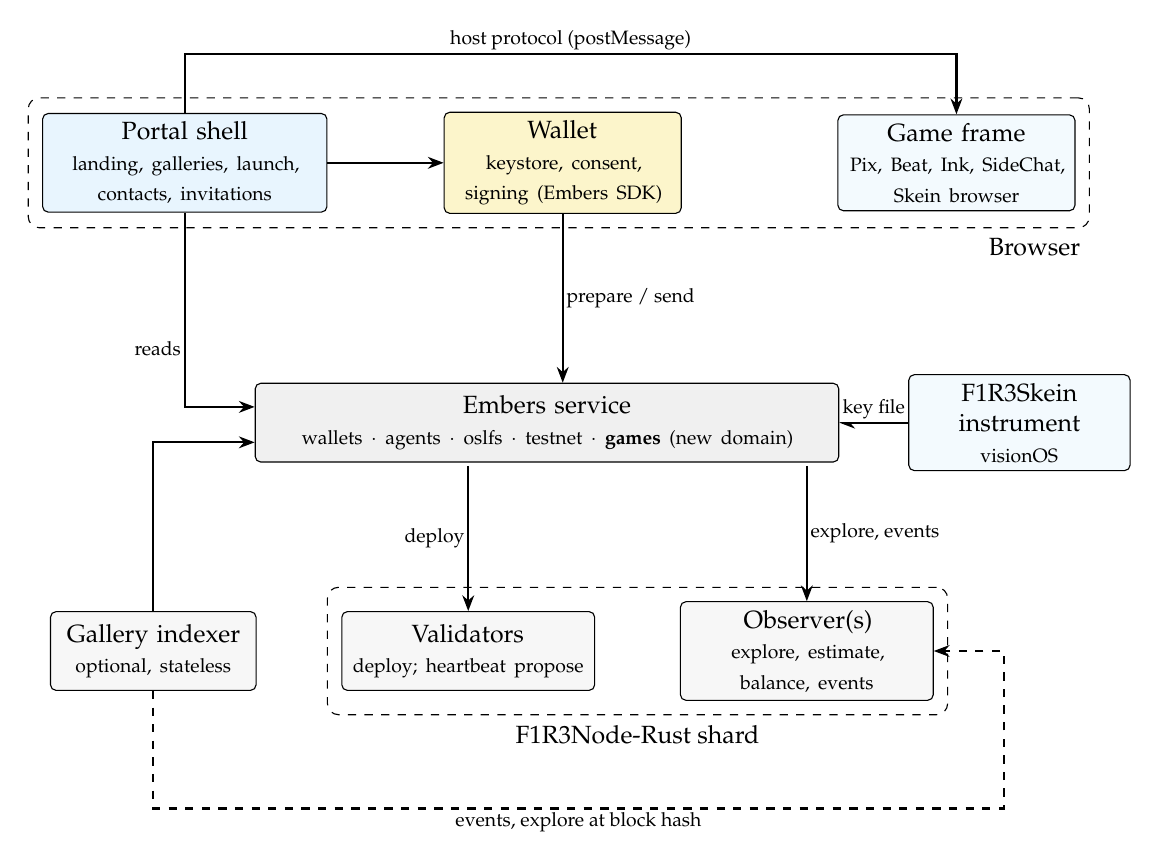
\begin{tikzpicture}[
  box/.style={draw, rounded corners=2pt, align=center, font=\small,
              minimum height=10mm, inner sep=3pt},
  grp/.style={draw, dashed, rounded corners=4pt, inner sep=5pt},
  arr/.style={-{Stealth[length=2mm]}, thick},
  lab/.style={font=\scriptsize, fill=white, inner sep=1pt}
]
\node[box, fill=sky!12, text width=34mm] (shell) at (0,0) {Portal shell\\\scriptsize landing, galleries, launch, contacts, invitations};
\node[box, fill=ylw!25, text width=28mm] (wallet) at (4.8,0) {Wallet\\\scriptsize keystore, consent, signing (Embers SDK)};
\node[box, fill=sky!6, text width=28mm] (game) at (9.8,0) {Game frame\\\scriptsize Pix, Beat, Ink, SideChat, Skein browser};
\node[grp, fit=(shell)(wallet)(game), label={[font=\small,anchor=north east]south east:Browser}] (br) {};
\node[box, fill=black!6, text width=72mm] (em) at (4.6,-3.3) {\Em{} service\\\scriptsize wallets $\cdot$ agents $\cdot$ oslfs $\cdot$ testnet $\cdot$ \textbf{games} (new domain)};
\node[box, fill=sky!6, text width=26mm] (avp) at (10.6,-3.3) {F1R3Skein instrument\\\scriptsize visionOS};
\node[box, fill=black!3, text width=30mm] (val) at (3.6,-6.2) {Validators\\\scriptsize deploy; heartbeat propose};
\node[box, fill=black!3, text width=30mm] (obs) at (7.9,-6.2) {Observer(s)\\\scriptsize explore, estimate, balance, events};
\node[grp, fit=(val)(obs), label={[font=\small]below:\Nd{} shard}] (sh) {};
\node[box, fill=black!3, text width=24mm] (idx) at (-0.4,-6.2) {Gallery indexer\\\scriptsize optional, stateless};

\draw[arr] (shell) -- (wallet);
\draw[arr] (shell.north) -- ++(0,0.75) -| node[lab, pos=0.25, above]{host protocol (postMessage)} (game.north);
\draw[arr] (wallet.south) -- node[lab, right]{prepare / send} (wallet.south |- em.north);
\draw[arr] (shell.south) |- node[lab, pos=0.35, left]{reads} ($(em.west)+(0,0.2)$);
\draw[arr] (3.6,-3.3) ++(0,-0.55) -- node[lab, left]{deploy} (val.north);
\draw[arr] (7.9,-3.3) ++(0,-0.55) -- node[lab, right]{explore, events} (obs.north);
\draw[arr] (avp.west) -- node[lab, above]{key file} (em.east);
\draw[arr] (idx.north) |- ($(em.west)+(0,-0.25)$);
\draw[arr, dashed] (idx.south) -- (-0.4,-8.2) -- node[lab, below]{events, explore at block hash} (10.4,-8.2) |- (obs.east);
\end{tikzpicture}
\caption{Components. The browser never holds a server session and never talks to a
validator; it talks to \Em{}, which renders, deploys and reads. The shard holds the \code{games} environment, the games' own environments and \code{SystemVault}. Solid arrows are
requests.}
\label{fig:arch}
\end{figure}

\subsection{Components}

\begin{longtable}{@{}>{\raggedright\arraybackslash}p{0.22\textwidth}>{\raggedright\arraybackslash}p{0.72\textwidth}@{}}
\toprule
Component & Responsibility\\
\midrule
\endhead
Portal shell & A React web application (as \Sky{} is), served as static files.
Landing, sign-on, dashboard of games, galleries, launch, the contact dialogue,
invitation redemption, and the host side of the game protocol.\\
Wallet & A module of the shell, isolated behind a narrow interface. Holds the
encrypted keystore, decides consent, signs with the \Em{} SDK, and calls \Em{}'s
wallets domain for balance, history and transfers.\\
Game frame & Each web game runs in a sandboxed frame on its own origin and reaches
identity, payment and the shard only through the host protocol
(\S\ref{sec:hostproto}).\\
\Em{} \code{games} domain & New. Endpoints and templates for profiles, the game
registry, instances, play records, invitations and engagement, built as \Em{}'s other
domains are; deploys and maintains the \code{games} environment.\\
\Em{} (existing) & Wallets (balance, history, transfers), testnet faucet, and the
node clients and event subscriptions every domain shares.\\
Gallery indexer & Optional. Rebuilds ordered gallery views from \code{/ws/events}
and exploratory reads, for scale; everything it returns carries the block hash it
read at, so a client can check it against an observer.\\
\Nd{} shard & Validators accept deploys and propose by heartbeat; observers serve
every read and the event stream.\\
\bottomrule
\end{longtable}

\subsection{Why an \Em{} domain and not a new service}

The design of the earlier F1R3Skein development plan proposed a new
\code{f1r3games-service} ``modelled on \Em{}''. Conformance argues for going the
whole way: a domain inside \Em{} inherits, without reimplementation, the node
clients and their configuration, the environment-key handling, the prepare/send
token, typed rendering, the event subscriptions, the OpenAPI schema from which the
client SDK is generated, and the deployment. The Portal then uses one SDK for its
wallet and its games, as \Sky{} uses one SDK for its wallet and agents. Whether the
domain lives in the \Em{} repository or in a crate that \Em{} links is Open
decision~\ref{dec:home}; the protocol is the same either way.

%======================================================================
\section{Identity and sign-on}\label{sec:identity}

\subsection{The key and the address}

A person's identity is one secp256k1 key pair. The public key, hex encoded
uncompressed, is the \code{deployer} of every deploy the person makes; the address
is the F1R3Cap address the \Em{} SDK derives from it, which is also the address of
the person's vault in \code{SystemVault}. The Portal \MUST{} obtain both from the
SDK (\code{PrivateKey}, \code{getPublicKey()}, \code{getAddress()}) and \MUSTNOT{}
reimplement the derivation.

\subsection{Creating, importing and exporting}

\begin{description}[leftmargin=*,itemsep=2pt]
\item[Create.] \code{PrivateKey.new()}; then, before the person can continue, the
  Portal offers the key file for download exactly as \Sky{} does
  (\code{<address>.json}, \code{serializeKey}). The Portal does not let a person
  proceed past creation without either downloading the file or explicitly
  acknowledging that losing the device loses the key.
\item[Import.] Upload of a \Sky{} key file (\code{deserializeKey}), or paste of the
  64-hex-digit value.
\item[Export.] The same file, on request, after re-unlocking.
\end{description}

A key created in the Portal \MUST{} open in \Sky{} and in \Gz{}, and vice versa;
this is an acceptance test (\S\ref{sec:accept}).

\subsection{The keystore}\label{sec:keystore}

\Sky{} keeps keys only in memory. The Portal must keep the person signed on across
visits, so it keeps an encrypted keystore in the browser's IndexedDB:

\begin{itemize}[leftmargin=*,itemsep=2pt]
\item Each entry is the \Sky{} key file encrypted with AES-256-GCM under a wrapping
  key, with the address and a label in clear.
\item The wrapping key is derived either from a passphrase (PBKDF2-SHA-256 through
  WebCrypto, with a stored salt and a calibrated iteration count) or from a passkey
  using the WebAuthn PRF extension where the browser supports it (Open
  decision~\ref{dec:unlock}).
\item Unlocked, the decrypted key lives only in the wallet module's memory, for a
  configurable idle period, after which the wallet locks.
\item Several keys may be held; one is \emph{active} and pays. This is \Gz{}'s model
  and lets a person keep separate identities.
\end{itemize}

\subsection{What ``signed on'' means}

There is no login server. \Em{} is stateless and authenticates every write by the
signature on the deploy it prepared; reads are public. Being signed on is therefore
a client state: an unlocked active key, and the person's profile read from the
\code{games} environment. Single sign-on across games follows from the games never
holding keys: a game asks the shell, and the shell's wallet signs
(\S\ref{sec:hostproto}). Nothing has to be shared between game origins except the
protocol.

\subsection{Profiles}

A profile is a small record in the \code{games} environment keyed by address:
display name, a sigil seed (the avatar is computed from the address, as in the
prototype, so the seed is only a variation), optional tags, and creation and
last-seen times. It is written by \code{profiles/save} and only the owner's deploy
can write it. A person with no profile is still a valid player, shown by address and
sigil.

%======================================================================
\section{The wallet}\label{sec:wallet}

\subsection{Functions}

\begin{longtable}{@{}>{\raggedright\arraybackslash}p{0.22\textwidth}>{\raggedright\arraybackslash}p{0.72\textwidth}@{}}
\toprule
Function & Implementation\\
\midrule
\endhead
Balance and history & \Em{} \code{GET /wallets/:address/state}; live updates from
\code{GET /wallets/:address/deploys}.\\
Receive & Show the address and a QR code.\\
Send & \Em{} \code{/wallets/transfer/prepare}, verify, sign, \code{/send}.\\
Game spending & Per game and per instance, the phlo costs of deploys the person made
there, read from the deploy records.\\
Consent & Every signature, except within an allowance, is preceded by a prompt naming
the game, the action, the paying address and its balance, and the quoted cost.\\
Allowances & A per-instance budget within which a game's registered templates are
signed without prompting (\S\ref{sec:allowance}).\\
Keys & Create, import, export, label, choose active, remove.\\
\bottomrule
\end{longtable}

\subsection{Signing rules}\label{sec:signrules}

The wallet adopts \Gz{}'s rules (Finding~\ref{f:gaze}), restated against \Em{}'s
protocol:

\begin{enumerate}[leftmargin=*,itemsep=2pt]
\item \textbf{Decode strictly.} The prepared bytes \MUST{} decode as one
  \code{DeployData} with each field once, canonically encoded; the \code{shardId}
  \MUST{} equal the configured shard.
\item \textbf{Cap the fee.} \code{phloPrice}~$\times$~\code{phloLimit} \MUST{} be
  within the person's fee cap, and within the remaining allowance if signing without
  a prompt.
\item \textbf{Recognise the term.} The term \MUST{} equal a registered template
  (the Portal's own, or one listed by hash in the game's manifest) rendered with the
  values the request named. The wallet re-renders the template locally from the
  same typed values and compares; any difference refuses.
\item \textbf{No deployer authority to games.} A game template \MUSTNOT{} bind
  \code{rho:system:deployerId}, \code{rho:system:deployerId:ops} or
  \code{rho:vault:system} directly; these are reachable only through the
  \code{games} environment's methods, whose code is fixed and audited. Only the
  wallet's own transfer template touches the vault.
\item \textbf{Quote the cost.} Before prompting, the cost is estimated by \Em{}
  through \code{POST /api/estimate-cost} on an observer, passing the deployer key so
  identity-dependent terms are quoted correctly (\code{docs/node/api-reference.md}).
\end{enumerate}

Rule~3 requires the client and \Em{} to render identically. The \code{games} domain
\MUST{} publish each template and its renderer's literal rules, and the wallet
\MUST{} implement \code{firefly-client}'s \code{Value} rendering in TypeScript,
tested against vectors produced by the Rust renderer (Obligation~\ref{ob:render}).

\subsection{Allowances}\label{sec:allowance}

Games such as F1R3Pix make many small moves; a prompt per move is unusable. On
launching or joining an instance, the wallet offers an allowance: a phlo budget, an
expiry, and the set of template hashes the game's manifest declares for play. Within
it the wallet signs without prompting, still applying every rule of
\S\ref{sec:signrules}, and shows a running total. On \code{master} the allowance is
enforced only by the wallet; the person's whole balance remains at risk only from the
wallet's own code, which is the same trust \Sky{} asks for.

When offered-funded deploys reach \code{master} (Finding~\ref{f:branch}), an
allowance becomes a private purse funded by \code{SystemVault.transferBatch} and
named in each move's signed funding intent, so the budget is enforced by the shard
and the person's main balance is not exposed to a game at all. The protocol to games
does not change.

%======================================================================
\section{The \code{games} environment on the shard}\label{sec:env}

\subsection{Shape}

The \code{games} domain deploys one environment, in \Em{}'s pattern: a registry
entry inserted with \code{rho:registry:insertSigned:secp256k1} under the
\code{games\_env\_key}, holding \code{(version, bundle+\{*games\})}, re-initialised
only when the deployed version is lower. Within it, one dispatch contract
\code{games(@method, ...)} and state in \code{treeHashMap}s. Every write method begins
by deriving the caller's address:

\begin{lstlisting}[language=Rho]
new deployData(`rho:deploy:data`), vaultAddress(`rho:vault:address`),
    deployDataCh, callerCh in {
  deployData!(*deployDataCh) |
  for (_, @deployerId, _ <- deployDataCh) {
    vaultAddress!("fromDeployerId", deployerId, *callerCh)
  } |
  for (@caller <- callerCh) { /* authorise against caller */ }
}
\end{lstlisting}

\subsection{Domains and methods}

\begin{longtable}{@{}>{\raggedright\arraybackslash}p{0.16\textwidth}>{\raggedright\arraybackslash}p{0.4\textwidth}>{\raggedright\arraybackslash}p{0.36\textwidth}@{}}
\toprule
Domain & Methods & Authorisation\\
\midrule
\endhead
profiles & \code{save}, \code{get}, \code{list} & owner writes; anyone reads\\
registry & \code{register}, \code{update}, \code{retire}, \code{get}, \code{list}
  & operator key (later, governance); anyone reads\\
instances & \code{create}, \code{join}, \code{leave}, \code{setStatus},
  \code{get}, \code{listByGame}, \code{listByPlayer} & host creates; join by
  invitation or, for public instances, by anyone; host and game sets status\\
plays & \code{publish}, \code{saveVersion}, \code{get}, \code{list},
  \code{link} & participants of the instance publish; anyone reads\\
invitations & \code{issue}, \code{redeem}, \code{revoke}, \code{status}
  & participants issue; holder of the invitation secret redeems; issuer revokes\\
engagement & \code{record}, \code{counts} & any address, once per (address, play,
  kind) for kinds that count people\\
\bottomrule
\end{longtable}

\subsection{Instances}

An instance is created by one deploy that \code{new}s an unforgeable name for it. The
client learns that name before deploying, from \code{POST /api/prepare-deploy}
(Finding~\ref{f:prepare}), which \Em{}'s \code{instances/create/prepare} calls, so
the Portal can show the instance, its link and its invitations before the deploy is
finalised. The instance record is:

\begin{lstlisting}[language=Json]
{ "id": <hex of the unforgeable name>, "game": "f1r3pix",
  "host": <address>, "createdAt": <ms>, "visibility": "public" | "unlisted" | "private",
  "status": "lobby" | "active" | "closed",
  "participants": { <address>: { "role": "host" | "player" | "reader",
                                 "joinedAt": <ms> } },
  "gameEnv": <registry URI of the game's own environment>,
  "gameRef": <the game's handle for this instance's state> }
\end{lstlisting}

The game's own state for the instance lives in the game's environment, not in
\code{games}. The \code{create} deploy calls the game's environment to initialise
it (its \code{init} method, named in the manifest) and records the handle it returns.
This fixes the mistake of global per-game state (Finding~\ref{f:mistakes}, item~5)
at the point of creation: a game that cannot initialise a fresh instance cannot be
registered.

\subsection{Play records}

A play record follows \Em{}'s versioned-record shape: a header, small and listable,
and a body, possibly large, kept under versions with a \code{"latest"} alias.

\begin{lstlisting}[language=Json]
header: { "id", "game", "kind", "instance", "authors": [<address>],
          "title", "createdAt", "preview": <small, kind-specific>,
          "bodyHash": <blake2b-256 of the body>, "links": [<play id>] }
body:   <kind-specific: a pixel grid, a beat pattern, an ink set,
         a story's beats, a skein tune term, a performance trace>
\end{lstlisting}

\code{list} projects headers only. The \code{kind} is declared by the game's
manifest: one kind for most games, two for F1R3Skein (\code{tune},
\code{performance}), linked in both directions through \code{links} (a tune names
the performance it was snipped from; a performance names the tunes harvested from
it). Bodies too large for the chain are stored by hash in F1R3Drive and only their
hash recorded (Open decision~\ref{dec:bodies}).

\subsection{Ordering and paging}

Gallery views need recency and engagement order. The environment keeps, per game and
kind, a time-bucketed index (\code{treeHashMap} from day number to the list of play
ids published that day), and \code{list} pages by bucket. Engagement order is
computed from \code{counts}. At small scale \Em{} serves both by exploratory deploys
on an observer; at larger scale the gallery indexer serves them, rebuilding from
\code{block-finalised} events and reads. Every page returned carries the block hash
it reflects. Paging cost is Obligation~\ref{ob:paging}.

\subsection{Rendering and injection}

Every template is rendered from typed values by \code{firefly-client}
(Finding~\ref{f:embers}). Free text from players (titles, names, tags) is passed as
\code{Value::String} and never spliced; byte payloads as \code{Value::Bytes}.
Templates \MUST{} contain no other interpolation.

%======================================================================
\section{Games}\label{sec:games}

\subsection{The game manifest}

A game is a manifest registered in the \code{games} registry. The manifest is JSON;
its hash is what the registry records, and the Portal fetches it from the game's
origin and checks the hash.

\begin{lstlisting}[language=Json]
{ "id": "f1r3pix", "name": "F1R3Pix", "tagline": "Collective Visual Intelligence",
  "entry": "https://pix.games.f1r3fly.io/", "platforms": ["web"],
  "env": "rho:id:...",                       // the game's own environment
  "init": { "template": "<hash>", "phloLimit": 200000 },
  "playTemplates": ["<hash>", "<hash>"],     // signable under an allowance
  "otherTemplates": ["<hash>"],              // always prompted
  "galleries": [ { "kind": "canvas", "renderer": "https://.../preview.html" } ],
  "contactsDialogue": true,
  "readerTier": true,
  "minProtocol": 1 }
\end{lstlisting}

The Portal's dashboard, galleries and launch flow are generated from the registry;
adding a game is registering a manifest (Requirement~\ref{req:open}).

\subsection{The host protocol}\label{sec:hostproto}

A web game runs in a sandboxed frame on its own origin. It speaks to the shell by
\code{postMessage}, with the shell checking the frame's origin against the manifest's
\code{entry}. Version 1:

\begin{longtable}{@{}>{\raggedright\arraybackslash}p{0.26\textwidth}>{\raggedright\arraybackslash}p{0.68\textwidth}@{}}
\toprule
Message (game $\to$ shell) & Effect\\
\midrule
\endhead
\code{hello\{protocol\}} & Shell replies with the person's address, profile,
  sigil seed, and the instance context (id, role, participants, \code{gameRef}).\\
\code{deploy\{template, values\}} & The wallet renders, applies
  \S\ref{sec:signrules}, prompts or uses the allowance, signs, and sends through \Em{};
  replies with the deploy id, then its finalisation.\\
\code{read\{template, values\}} & An exploratory read through \Em{} at an observer;
  replies with the value and block hash.\\
\code{estimate\{template, values\}} & Cost quote only.\\
\code{publishPlay\{kind, title, preview, body, links\}} & Shell prepares
  \code{plays/publish}; same signing path.\\
\code{invite\{\}} & Opens the shared contact and invitation dialogue
  (\S\ref{sec:invite}) over the game; refused for games whose manifest sets
  \code{contactsDialogue: false}.\\
\code{engage\{play, kind\}} & Records engagement.\\
\code{subscribe\{events\}} & Forwards finalisation events relevant to the
  instance.\\
\midrule
Message (shell $\to$ game) & \\
\midrule
\code{context}, \code{event}, \code{locked} & Context changes, forwarded events,
  wallet locked (game should pause signing).\\
\bottomrule
\end{longtable}

The game never sees a key and never constructs a deploy the wallet has not rendered
itself.

\subsection{Launch}

\begin{figure}[ht]
\centering
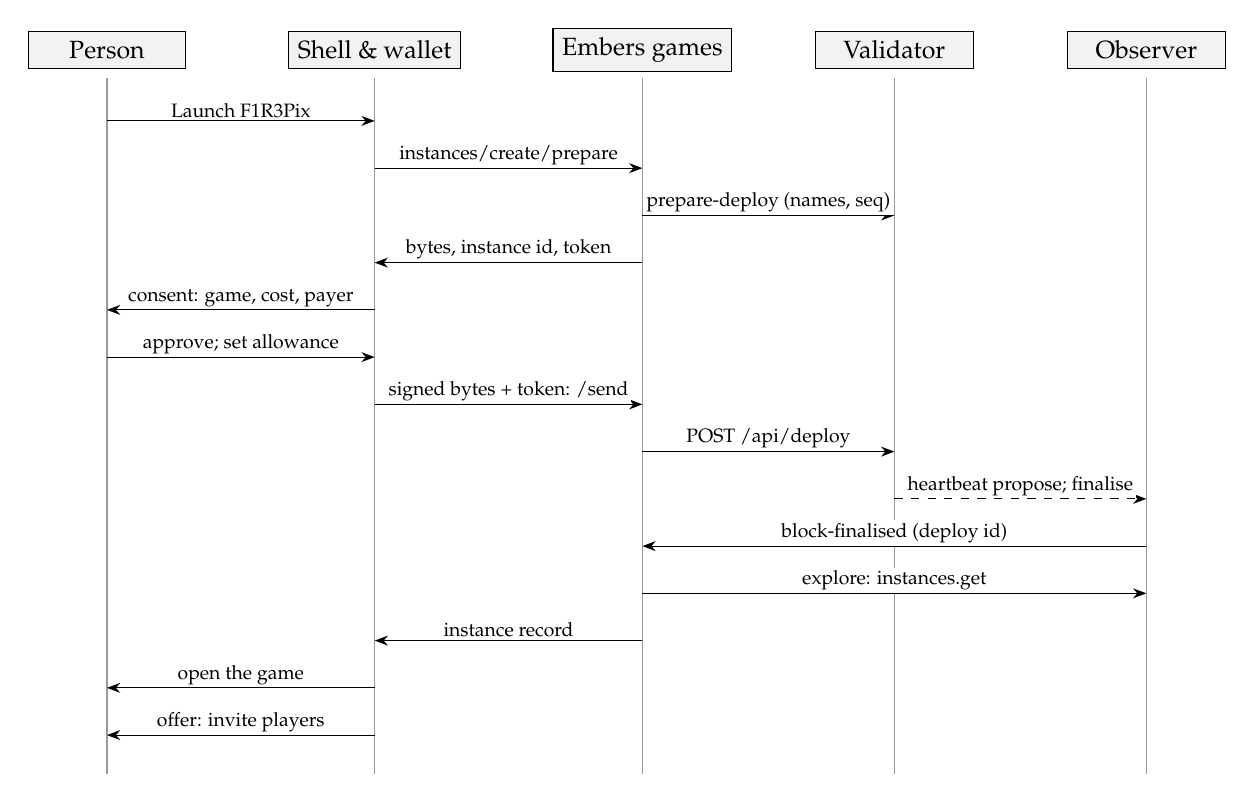
\begin{tikzpicture}[font=\small, >=Stealth]
\def\H{9.2}
\foreach \x/\n in {0/Person, 3.4/Shell \& wallet, 6.8/\Em{} games, 10/Validator, 13.2/Observer}{
  \node[draw, fill=black!5, minimum width=20mm, align=center] at (\x,0) {\n};
  \draw[black!40] (\x,-0.35) -- (\x,-\H);
}
\newcommand{\msg}[4]{\draw[->] (#1,-#3) -- node[above, font=\scriptsize, fill=white, inner sep=1pt]{#4} (#2,-#3);}
\msg{0}{3.4}{0.9}{Launch F1R3Pix}
\msg{3.4}{6.8}{1.5}{instances/create/prepare}
\msg{6.8}{10}{2.1}{prepare-deploy (names, seq)}
\msg{6.8}{3.4}{2.7}{bytes, instance id, token}
\msg{3.4}{0}{3.3}{consent: game, cost, payer}
\msg{0}{3.4}{3.9}{approve; set allowance}
\msg{3.4}{6.8}{4.5}{signed bytes + token: /send}
\msg{6.8}{10}{5.1}{POST /api/deploy}
\draw[->, dashed] (10,-5.7) -- node[above, font=\scriptsize, fill=white, inner sep=1pt]{heartbeat propose; finalise} (13.2,-5.7);
\msg{13.2}{6.8}{6.3}{block-finalised (deploy id)}
\msg{6.8}{13.2}{6.9}{explore: instances.get}
\msg{6.8}{3.4}{7.5}{instance record}
\msg{3.4}{0}{8.1}{open the game}
\msg{3.4}{0}{8.7}{offer: invite players}
\end{tikzpicture}
\caption{Launching an instance. The instance id is known at step~4, before the
deploy, from \code{prepare-deploy}.}
\label{fig:launch}
\end{figure}

\subsection{The games}

\begin{longtable}{@{}>{\raggedright\arraybackslash}p{0.15\textwidth}>{\raggedright\arraybackslash}p{0.26\textwidth}>{\raggedright\arraybackslash}p{0.27\textwidth}>{\raggedright\arraybackslash}p{0.24\textwidth}@{}}
\toprule
Game & An instance is & A play record is & Integration\\
\midrule
\endhead
F1R3Pix & one shared canvas & the canvas at close, or a snapshot the players mark &
  web; contacts dialogue\\
F1R3Beat & one evolving pattern session & a pattern and its lineage & web;
  contacts dialogue; engagement feeds selection\\
F1R3Ink & one group colouring round & the set of inks given and received & web;
  contacts dialogue\\
F1R3SideChat & one story & arcs and beats; readers browse without a key
  (\code{readerTier}) & web; contacts dialogue\\
F1R3Skein & one performance session & two kinds: \code{performance} (the
  gesture trace) and \code{tune} (a snipped term), cross-linked & Vision Pro
  instrument plus web browser; the browser sets \code{contactsDialogue: false};
  engagement feeds selection\\
\bottomrule
\end{longtable}

Each game is rebuilt against this protocol and its own environment; the existing
per-game \code{Shard/} services are research, not a base (Finding~\ref{f:mistakes}).

\subsection{F1R3Skein on Vision Pro}

The instrument is not a web frame. It imports the person's key file (the \Sky{}
format, by AirDrop or file picker) into the device keychain, signs with the same
deploy encoding, and calls the same \Em{} \code{games} endpoints, following the same
signing rules. A Portal instance page shows a QR code and a universal link carrying
the instance id, which the instrument opens to join the session and to publish
performances and tunes into it.

%======================================================================
\section{Galleries}\label{sec:gallery}

\subsection{What the person sees}

From the dashboard, each game card offers \emph{Launch} and \emph{Gallery}; a
\emph{Feed} tab interleaves all games. A gallery is an endlessly scrolling list of
play headers, filterable by game, kind, participant and date, and sortable by
recency, engagement, and (for kinds that have lineage) depth. Opening a play shows
its preview rendered by the game's sandboxed renderer, its participants, its links
(for F1R3Skein, ``hear this in context'' from a tune and ``tunes harvested here''
from a performance) and its engagement counts, with \emph{open in game} where the
game supports it.

\subsection{No sign-on to read}

Galleries are read through \Em{} with no key: every read is an exploratory deploy on
an observer, which costs no phlo. This also gives SideChat its free reader tier. A
person who is not signed on sees an invitation to create a key at the point of first
engagement, not before.

\subsection{Trust in the view}

Every page carries the block hash it was read at. A client \MAY{} spot-check any
header by its own exploratory read on an observer at that hash
(\code{explore-deploy-by-block-hash}), so neither \Em{} nor the indexer can forge a
gallery undetected.

%======================================================================
\section{Contacts and invitations}\label{sec:invite}

\subsection{Sharing contacts with the Portal}

The contact dialogue is the prototype's, rebuilt as one component used by every game
whose manifest allows it.

\begin{description}[leftmargin=*,itemsep=2pt]
\item[Sources.] A vCard or CSV file the person exports from her address book; the
  browser Contact Picker API where available (it returns only the entries the person
  selects); handles typed by hand for email, Discord, Slack, Mattermost, Telegram and
  others; and the addresses of players she has already played with, read from
  instance records.
\item[Consent.] Each import says what will be kept and where. Nothing is imported in
  the background, and nothing is read from an account by OAuth in this version.
\item[Storage.] Contacts are kept in IndexedDB, encrypted with AES-256-GCM under a key
  derived from the active private key by HKDF with a fixed, versioned context string,
  so the same contact book opens on any device that holds the key.
\item[Backup.] Optional: the encrypted contact book, padded to a size bucket, saved as
  a private record in the \code{games} environment, whose ciphertext only the key
  holder can read (\Em{} already stores encrypted payloads for agent teams). Open
  decision~\ref{dec:backup}.
\item[Deletion.] Removing a contact removes it locally and from the next backup.
\end{description}

No contact's name, handle or email ever appears in a deploy, a template, a log or an
\Em{} request. The Portal does not try to discover which contacts already play:
hashed identifiers are guessable, and the invitation itself is the discovery.

\subsection{The invitation}

An invitation is a fresh secp256k1 key pair made by the inviter's wallet for that
invitation: the \emph{invite key}. Its public key is recorded on the shard; its
private key travels to the invitee inside the link's fragment, which browsers do not
send to servers:

\begin{lstlisting}
https://games.f1r3fly.io/i/<instance id>#<invite private key, base64url>
\end{lstlisting}

\code{invitations/issue} records, under the invite public key: the instance, the
issuer, the number of uses (one per invitee by default; more for an open link), an
expiry block height, and an optional \emph{stipend} from the issuer to each new
player. To redeem, the invitee's wallet signs the invitee's own address with the
invite key and deploys \code{invitations/redeem} with that signature; the contract
checks it with \code{rho:crypto:secp256k1Verify}, so a copy of a pending redeem deploy
cannot be re-used by another address, decrements the uses, adds the invitee to the
instance, and pays the stipend. Appendix~\ref{app:rho} sketches the contract.

This uses only \code{master} primitives. When \code{rho:system:capabilities} reaches
\code{master}, \code{issue} can register a bounded-use capability keyed by the invite
public key, and the link format stays the same.

\subsection{Delivery}\label{sec:delivery}

The Portal composes a message per invitee (game, instance, inviter's name, link) and
delivers it through the person's own channels: the system share sheet (Web Share
API), \code{mailto:}, copy to clipboard, or a QR code. The operator sends nothing on
the person's behalf in this version. Relays through F1R3MTA or the F1R3FLY bot
gateway are possible later; neither may put the recipient or the message on chain.

\subsection{Redemption}

\begin{figure}[ht]
\centering
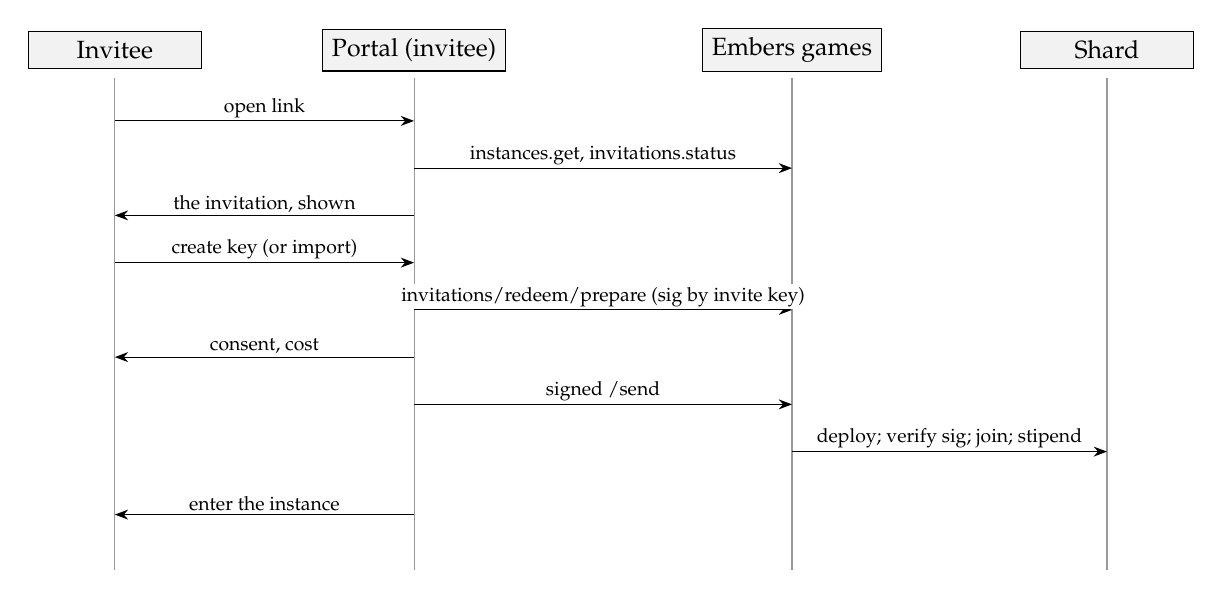
\begin{tikzpicture}[font=\small, >=Stealth]
\def\H{6.6}
\foreach \x/\n in {0/Invitee, 3.8/Portal (invitee), 8.6/\Em{} games, 12.6/Shard}{
  \node[draw, fill=black!5, minimum width=22mm, align=center] at (\x,0) {\n};
  \draw[black!40] (\x,-0.35) -- (\x,-\H);
}
\newcommand{\msg}[4]{\draw[->] (#1,-#3) -- node[above, font=\scriptsize, fill=white, inner sep=1pt]{#4} (#2,-#3);}
\msg{0}{3.8}{0.9}{open link}
\msg{3.8}{8.6}{1.5}{instances.get, invitations.status}
\msg{3.8}{0}{2.1}{the invitation, shown}
\msg{0}{3.8}{2.7}{create key (or import)}
\msg{3.8}{8.6}{3.3}{invitations/redeem/prepare (sig by invite key)}
\msg{3.8}{0}{3.9}{consent, cost}
\msg{3.8}{8.6}{4.5}{signed /send}
\msg{8.6}{12.6}{5.1}{deploy; verify sig; join; stipend}
\msg{3.8}{0}{5.9}{enter the instance}
\end{tikzpicture}
\caption{Redeeming an invitation. The invite key never leaves the invitee's browser; only its signature over the invitee's address is deployed.}
\label{fig:redeem}
\end{figure}

\subsection{Paying for a newcomer's first deploy}\label{sec:stipend}

A new key has an empty vault, and the redeem deploy costs phlo. Three routes, in order
of preference:

\begin{enumerate}[leftmargin=*,itemsep=2pt]
\item \textbf{Testnets and local shards:} \Em{}'s testnet faucet (\code{POST
  /testnet/wallet}) funds the new address before redemption; ign1t10n's genesis funds
  the local operator.
\item \textbf{The inviter pays first:} \code{issue} accepts a stipend escrow; at
  invitation time the Portal also offers to transfer a small amount directly to a
  \emph{fresh} address it pre-generates for the invitee and places in the fragment
  alongside the invite key, so the invitee's first key is already funded. (The
  invitee is told this key was made by the inviter and is offered to rotate to a new
  one, funded by transfer, at once.)
\item \textbf{After offered funding reaches \code{master}:} the redeem deploy is
  funded from the invitation's private purse, and no pre-generated key is needed.
\end{enumerate}

Which route production uses is Open decision~\ref{dec:stipend}.

%======================================================================
\section{Engagement}\label{sec:engagement}\label{sec:engagementsec}

\code{engagement/record} counts plays, likes, opens, tips (as a link to a wallet
transfer) and game-specific signals declared in the manifest (for F1R3Skein,
\emph{snipped-from} and \emph{bred-from}). Kinds that count people are limited to one
per address per play. The Portal shows the counts; the games read them to drive
selection. Weighting and resistance to gaming are the games' concern
(\S\ref{sec:scope}), and the counts are public so that any weighting can be audited.

%======================================================================
\section{Security and privacy}\label{sec:security}

\begin{longtable}{@{}>{\raggedright\arraybackslash}p{0.27\textwidth}>{\raggedright\arraybackslash}p{0.67\textwidth}@{}}
\toprule
Threat & Mitigation\\
\midrule
\endhead
Script injection in the shell & Strict Content Security Policy; no third-party
  script; the wallet module exposes only render-sign-send behind the rules of
  \S\ref{sec:signrules}; keystore encrypted at rest; idle lock.\\
A malicious or buggy game & Sandboxed frame on its own origin; no key access; only
  registered templates; no deployer authority in game templates; allowances bound
  spend.\\
A dishonest \Em{} & Cannot sign; cannot alter a prepared deploy undetected (the wallet
  re-renders and compares); can at worst refuse service or waste a capped fee. Reads
  are spot-checkable by block hash.\\
A dishonest indexer & Same as reads from \Em{}.\\
Front-running a redemption & Redemption is a signature over the redeemer's address;
  copying it helps no other address.\\
Leaked invitation link & Bounded uses and expiry; issuer can revoke; the link grants
  entry to one instance and a stipend, nothing more.\\
Spam invitations & Issuing costs the issuer phlo; delivery is through the issuer's own
  channels.\\
Lost device & The key file the person downloaded at creation; no operator recovery.
  Multi-signature vaults (\code{rho:vault:multiSig}) are a later option.\\
Rholang injection & Typed rendering only (\S\ref{sec:env}).\\
Linkability & One key links a person's plays across games; the wallet supports several
  keys and says so at creation.\\
Contact leakage & Contacts never leave the device unencrypted and never reach a
  deploy.\\
\bottomrule
\end{longtable}

%======================================================================
\section{Deployment}\label{sec:deploy}

\begin{longtable}{@{}>{\raggedright\arraybackslash}p{0.18\textwidth}>{\raggedright\arraybackslash}p{0.76\textwidth}@{}}
\toprule
Topology & Composition\\
\midrule
\endhead
Local & An ign1t10n shard (validators with heartbeat proposing, one observer),
  \Em{} with the \code{games} domain bound to it (ign1t10n can bundle \Em{}), and the
  Portal and games served from \code{localhost}. The testnet faucet funds new keys.\\
Testnet & An operator shard, \Em{}'s \code{testnet} configuration, the Portal at a
  public origin, faucet enabled.\\
Production & \Em{}'s \code{mainnet} configuration; faucet disabled; stipends from
  inviters.\\
\bottomrule
\end{longtable}

\Em{}'s configuration gains a \code{games\_env\_key}. The Portal's configuration names
the \Em{} base URL, the shard id, the fee cap default, and the games origins it will
frame.

%======================================================================
\section{The \Gz{} rendition}\label{sec:gaze}

\Gz{} keys and \Sky{} keys are the same files, so a person can carry one identity
into \Gz{} today. A later phase publishes the Portal as a shard site
(\code{f1r3://f1r3fly/games}) whose behaviour is f1r3lang, in which \Gz{}'s wallet
plays the part of the Portal's wallet and the host protocol maps onto capabilities
the page holds. Nothing in the \code{games} environment changes.

%======================================================================
\section{Testing and acceptance}\label{sec:accept}

\begin{enumerate}[leftmargin=*,itemsep=2pt]
\item A key created in the Portal opens in \Sky{} and \Gz{} and shows the same
  address; and conversely.
\item Two people on two browsers: one creates a key, launches an F1R3Pix instance and
  invites the other; the other redeems on a fresh browser with no key and plays; both
  see the same instance record and play record read from an observer.
\item A copied redeem deploy, re-signed by a third key, is rejected.
\item A game frame that asks to sign a term not in its manifest is refused without a
  prompt; one that exceeds its allowance gets a prompt.
\item A dishonest \Em{} that alters a prepared deploy's term or recipient is
  refused before signing.
\item Galleries load with no key; every page's block hash verifies against the
  observer.
\item F1R3Skein: a performance published from the instrument appears in the
  performance gallery with its tunes linked, and each tune links back.
\item The browser's network log shows no request to any server containing a
  contact.
\item No component in the Portal path calls propose.
\end{enumerate}

%======================================================================
\section{Work packages and schedule}\label{sec:plan}

\begin{longtable}{@{}>{\raggedright\arraybackslash}p{0.08\textwidth}>{\raggedright\arraybackslash}p{0.62\textwidth}>{\raggedright\arraybackslash}p{0.22\textwidth}@{}}
\toprule
WP & Content & Effort\\
\midrule
\endhead
W0 & Bring \Em{}'s templates to \code{master} system names; pin \Nd{},
  \Em{} and SDK versions; TypeScript port of \code{firefly-client} rendering with
  vectors. & 2 dev-weeks\\
W1 & Identity and wallet in the Portal: keystore, create/import/export, consent,
  signing rules, balance/history/transfer through \Em{}. & 3 dev-weeks\\
W2 & \Em{} \code{games} domain: environment, profiles, registry, instances (with
  prepare-deploy names), play records; regenerated SDK. & 4 dev-weeks\\
W3 & Portal shell: dashboard from the registry, launch, galleries, feed,
  spot-checking; host protocol v1. & 3 dev-weeks\\
W4 & Contacts and invitations: dialogue, encrypted store, invite keys, issue/redeem
  contract, stipends, faucet path. & 3 dev-weeks\\
W5 & First game ported: F1R3Pix (simplest state), end to end. & 2 dev-weeks\\
W6 & Remaining web games: Beat, Ink, SideChat (with reader tier). & 5 dev-weeks\\
W7 & F1R3Skein: browser galleries for tunes and performances; instrument key import
  and publishing. & 3 dev-weeks\\
W8 & Gallery indexer, engagement, security review, acceptance. & 3 dev-weeks\\
\bottomrule
\end{longtable}

W0--W5 (about 17 dev-weeks) yield a working Portal with one game; W6--W8 complete the
suite. Allowances by private purse and the \Gz{} rendition follow when their
dependencies land.

%======================================================================
\section{Obligations and decisions}\label{sec:open}

\subsection{Obligations}

\begin{obligation}[Name drift]\label{ob:drift}
Update \Em{}'s templates (\code{rho:rev:address} $\to$ \code{rho:vault:address} and
the deploy-identity names) and confirm the \code{rho:deploy:data} tuple shape on the
pinned \Nd{} revision; report the same drift to \Gz{}'s allow-list.
\end{obligation}

\begin{obligation}[Rendering parity]\label{ob:render}
Test vectors from \code{firefly-client} for every \code{Value} case, including
strings with quotes, backslashes, newlines and non-ASCII, matched byte for byte by
the TypeScript renderer.
\end{obligation}

\begin{obligation}[SDK]\label{ob:sdk}
Confirm how \code{@f1r3fly-io/embers-client-sdk} is published (\Sky{} pins
\code{\^{}0.0.79}; it is not on the public npm registry) and that its signing matches
the node's \code{secp256k1} verification for \code{DeployData} including
\code{shardId} and \code{expirationTimestamp}.
\end{obligation}

\begin{obligation}[Proposing]
Confirm heartbeat proposing on every target deployment and that \Em{}'s single
bootstrap propose is acceptable there.
\end{obligation}

\begin{obligation}[Paging]\label{ob:paging}
Measure \code{treeHashMap} bucket paging by exploratory deploy at 10\textsuperscript{4}
and 10\textsuperscript{5} plays per game; decide when the indexer becomes mandatory.
\end{obligation}

\begin{obligation}[Branch features]
Track \code{rho:system:capabilities} and offered-funded deploys on their way to
\code{master}; adopt each behind the existing interfaces when it arrives.
\end{obligation}

\subsection{Open decisions}

\begin{decision}[Home of the \code{games} domain]\label{dec:home}
Inside the \Em{} repository as a peer of \code{wallets} and \code{agents}, or a crate
\Em{} links. Proposed: inside, for one SDK and one deployment.
\end{decision}

\begin{decision}[Unlocking the keystore]\label{dec:unlock}
Passphrase only, or passkey (WebAuthn PRF) with passphrase fallback. Proposed: both.
\end{decision}

\begin{decision}[Large bodies]\label{dec:bodies}
Bodies above a threshold on chain anyway, or in F1R3Drive by hash. The F1R3MTA work
took bodies on chain; consistency argues the same, cost argues otherwise.
\end{decision}

\begin{decision}[Contact backup]\label{dec:backup}
Offer the encrypted on-shard backup in version~1, or keep contacts device-only.
\end{decision}

\begin{decision}[Stipends]\label{dec:stipend}
Default stipend amount, whether the pre-generated funded key of
\S\ref{sec:stipend} is offered in production, and whether the operator sponsors new
players at all.
\end{decision}

\begin{decision}[Registry governance]
Who may register and retire games: the operator key now, CatchingF1R3 governance
later?
\end{decision}

\begin{decision}[Default visibility]
Whether a new instance is public, unlisted or private by default, per game.
\end{decision}

%======================================================================
\appendix
\section{Sketch of the invitation methods}\label{app:rho}

Illustrative only; the implementation follows \Em{}'s template layout and is
rendered by \code{firefly-client}. \code{caller} is the address derivation of
\S\ref{sec:env}; \code{instances} and \code{invites} are \code{treeHashMap}s of the
environment; \code{currentBlock} reads \code{rho:block:data}.

\begin{lstlisting}[language=Rho]
contract games(@"invitations", @"issue", @invitePk, @instanceId,
               @uses, @expiresAt, @stipend, ret) = {
  new callerCh, okCh in {
    caller!(*callerCh) |
    for (@issuer <- callerCh) {
      isParticipant!(instanceId, issuer, *okCh) |
      for (@true <- okCh) {
        // stipend * uses is moved from the issuer's vault into the
        // environment's escrow vault (unforgeableAuthKey) in this deploy
        escrow!(issuer, stipend * uses, *okCh) |
        for (@true <- okCh) {
          treeHashMap!("set", invites, invitePk,
            { "instance": instanceId, "issuer": issuer, "uses": uses,
              "expiresAt": expiresAt, "stipend": stipend, "redeemed": Set() },
            *ret)
        }
      }
    }
  }
}

contract games(@"invitations", @"redeem", @invitePk, @sig, ret) = {
  new callerCh, invCh, hashCh, verifyCh, blockCh in {
    caller!(*callerCh) | currentBlock!(*blockCh) |
    treeHashMap!("get", invites, invitePk, *invCh) |
    for (@guest <- callerCh & @inv <- invCh & @height <- blockCh) {
      if (inv == Nil or height > inv.get("expiresAt") or inv.get("uses") <= 0
          or inv.get("redeemed").contains(guest)) { ret!((false, "invalid")) }
      else {
        blake2b256Hash!(guest.toByteArray(), *hashCh) |
        for (@digest <- hashCh) {
          secp256k1Verify!(digest, sig, invitePk, *verifyCh) |
          for (@true <- verifyCh) {
            treeHashMap!("set", invites, invitePk,
              inv.set("uses", inv.get("uses") - 1)
                 .set("redeemed", inv.get("redeemed").add(guest)), *devNull) |
            join!(inv.get("instance"), guest, "player", *devNull) |
            payStipend!(guest, inv.get("stipend"), *devNull) |
            ret!((true, inv.get("instance")))
          }
        }
      }
    }
  }
}
\end{lstlisting}

\section{Glossary}

\begin{description}[leftmargin=*,itemsep=1pt]
\item[Allowance] A budget within which the wallet signs a game's registered play
  templates without prompting.
\item[Environment] A versioned contract inserted in the registry by \Em{}, holding a
  domain's methods and state.
\item[Instance] One play of one game, created on the shard by its host.
\item[Invite key] A one-use key pair whose public half is recorded at issue and whose
  private half travels in the invitation link's fragment.
\item[Play record] A gallery entry: a listable header and a versioned body.
\item[Prepare / send] \Em{}'s two-step write: the server renders, the client signs.
\end{description}

\end{document}
